% Document class and font size
\documentclass[a4paper,10pt]{extarticle}

% Packages
\usepackage[utf8]{inputenc} % For input encoding
\usepackage{geometry} % For page margins
\geometry{a4paper, margin=0.75in} % Set paper size and margins
\usepackage{titlesec} % For section title formatting
\usepackage{enumitem} % For itemized list formatting
\usepackage{hyperref} % For hyperlinks
\usepackage{kotex}
\usepackage{graphicx}
\usepackage{array}
\usepackage{longtable}
\usepackage{float}
\usepackage[skip=3pt]{caption}

% Formatting
\setlist{noitemsep} % Removes item separation
\titleformat{\section}{\large\bfseries}{\thesection}{1em}{}[\titlerule] % Section title format
\titlespacing*{\section}{0pt}{\baselineskip}{\baselineskip} % Section title spacing
\graphicspath{{../../pictures}}

% Begin document
\begin{document}
% Disable page numbers
\pagestyle{empty}
% Enable page numbers
% \pagenumbering{arabic}

% Header

% \begin{minipage}{\textwidth}

\begin{minipage}{0.1\textwidth}
    \begin{flushleft}
        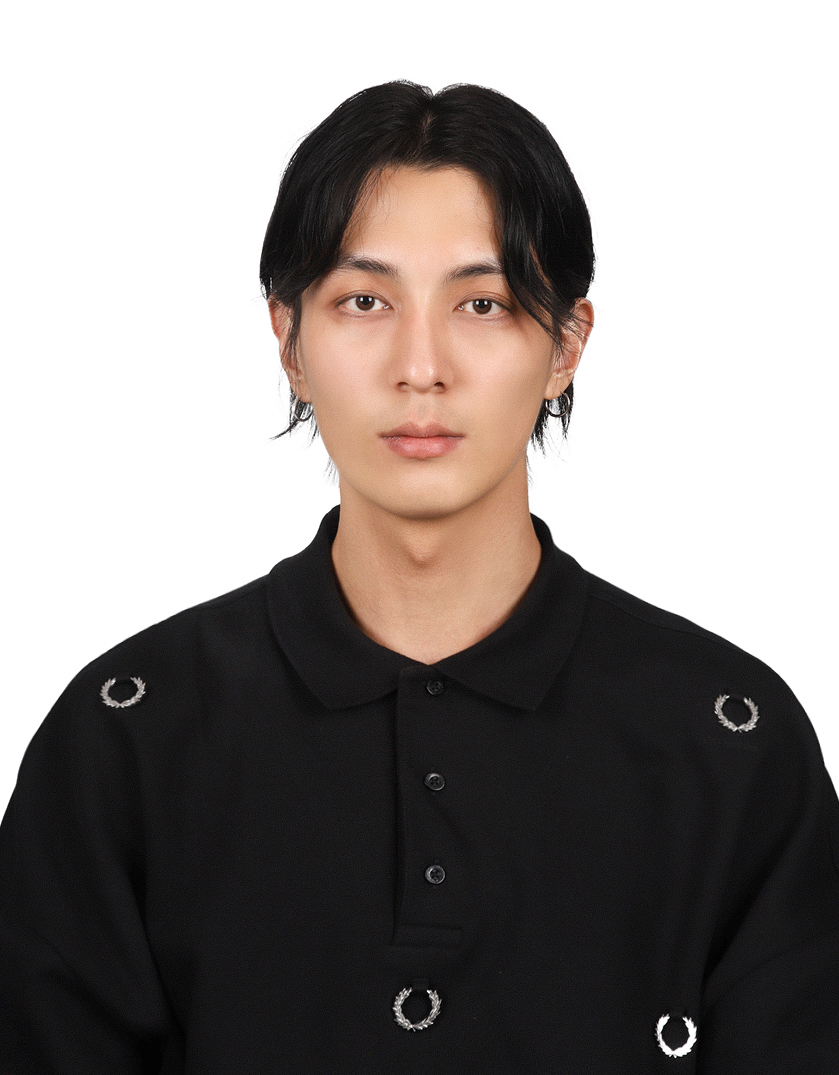
\includegraphics[height=3.5cm]{photo_231008.jpeg}
    \end{flushleft}
\end{minipage}
\hfill
\begin{minipage}{0.7\textwidth}
    \begin{flushright}
        \textbf{\Large 이현빈, Hyeonbeen Lee} % Name
        \newline\newline
        \begin{tabular}{rl}
            \textbf{Mobile: }    & +82-10-6236-4693                                                                                     \\
            \textbf{Instagram: } & \href{https://www.instagram.com/leehyeonbeen}{@leehyeonbeen}                                         \\
            \textbf{EMail: }     & \href{mailto:david.hyeonbeen.lee@gmail.com}{david.hyeonbeen.lee@gmail.com}                           
            % \textbf{LinkedIn: }  & \href{https://www.linkedin.com/in/hyeonbeen-lee-239500286/}{linkedin.com/in/hyeonbeen-lee-239500286} \\
            % \textbf{GitHub: }    & \href{https://github.com/hyeonbeenlee}{github.com/hyeonbeenlee}                                      \\
        \end{tabular}
        % \end{center}
    \end{flushright}

\end{minipage}
% \end{minipage}


% Education Section
\newcolumntype{L}{>{\raggedright\arraybackslash}m{1.6cm}}
\newcolumntype{R}{>{\centering\arraybackslash\small}m{3cm}}
\renewcommand*{\arraystretch}{1.5}
\noindent
\section*{인적사항}
\begin{center}
    \vspace*{-0.8cm}
    \noindent
    \begin{longtable}{LRLRLR}
        \textbf{성명:}   & 이현빈                                      & \textbf{생년월일:} & 1996.07.04 (양력)       & \textbf{경력여부:} & 신입         \\
        \hline
        \textbf{병역사항:} & 해병병장 만기전역 \small{(2017.05$\sim$2019.02)} & \textbf{주소:}   & 서울특별시 용산구 회나무로39길 6-3 & \textbf{지원분야:} & {오프라인 세일즈} \\
        \hline
        \textbf{신체사항: }& 189cm / 73kg & \textbf{언어:} & 한국어, 영어, 일본어
    \end{longtable}
\end{center}


% \textbf{성명}, 과학중점과정 \hfill 입학: 2012.03 | 졸업: 2015.02
% \newline
% \textbf{경희대학교}, 기계공학과 \hfill 입학: 2015.03 | 졸업: 2022.02\\ % University name and location
% 학사학위 (학위지도교수: 정신규, 김진균)\hfill 전체학점: 3.87/4.5 | 전공학점: 3.84/4.5\\ % Degree and GPA
% 학위논문명: \textit{\small{Data-driven aerodynamic coefficient prediction using}}\\
% \hspace*{1.9cm}\textit{\small{deep neural
%         network and PARSEC airfoil parameterization}}

% Education Section
\section*{학력사항}
\noindent
\textbf{반포고등학교}, 과학중점과정 \hfill 입학: 2012.03 | 졸업: 2015.02
\newline
\textbf{경희대학교}, 기계공학과 \hfill 입학: 2015.03 | 졸업: 2022.02\\ % University name and location
공학학사 (학위지도교수: 김진균, 정신규)\hfill 전체학점: 3.87/4.5 | 전공학점: 3.84/4.5 % Degree and GPA
% 학위논문명: \textit{\small{`Data-driven aerodynamic coefficient prediction using}}\\
% \hspace*{1.9cm}\textit{\small{deep neural
%         network and PARSEC airfoil parameterization'}}
\newline
\textbf{경희대학교 대학원}, 기계공학과 융합공학전공 \hfill 입학: 2022.03 | 졸업: 2024.02\\ % University name and location
공학석사 (학위지도교수: 김진균) \hfill 전체학점: 4.33/4.5 % Degree and GPA
% 학위논문명: \textit{\small{`Composite neural network with differential propagation}}\\
% \hspace*{1.9cm}\textit{\small{for modeling impulsive nonlinear dynamic systems'}}

\section*{지원 동기}
해외 디자이너 브랜드 리테일 세일즈 스태프 및 MD 구직중인 지원자 이현빈입니다. 공학석사학위를 취득하였으나, 삶에서 패션문화를 더 가까이 두며 살아가고자 지원하게 되었습니다.

공학계열 학사 및 석사 과정을 수학하며, 많은 전문지식 습득과 프로젝트 수행 및 논문출판에 따른 성취감을 느꼈습니다. 그랬던 저를 지금의 결정에 저를 도달하게 한 것은 과도한 업무량도 잦은 야근과 출장도 아닙니다. 제가 사랑하는 문화를 함께 향유할 사람이 없었다는 점입니다.

공학에 몸담으며 가장 힘겨웠던 점은 그런 주변 환경이었습니다. 함께 직접적으로 패션을 주제로 이야기하지 않아도, 서로가 서로를 알아채고 이해할 수 있는 사람들이 곁에 있어주길 바랬습니다. 나름대로 노력해보았지만, 업무에 치여 그럴 기회나 시간이 그리 많지 않았고 점차 웃는 날은 줄어가기만 했습니다.

일련의 시간과 생각들을 거쳐 졸업한 뒤로는 주변을 제가 좋아하는 것들로 채워나가기로 결정했습니다. 내가 좋아하는 것이니 재미있고 멋있기만 할 것이라는 헛된 기대나 환상을 품고 들어서지는 않았습니다. 주변에 패션업계나 세일즈 직무에 종사하는 친구들이 다들 각자 근무 스케줄이나 고객응대, 매장 내 대인관계로 힘들어하는 모습들도 보았습니다. 하지만 모두가 자신의 일을 사랑한다고 답합니다. 퇴근할 때에는 웃으며 동료들과 함께 돌아가는 모습을 보았습니다.
그런 사소할 수 있는 순간들이 모여 삶을 이룬다고 생각합니다. 제 자신에게 내린 답은, 주변에 어떤 빛깔의 사람들이 있고 어떤 색의 환경인지, 그곳에서 스스로의 만족을 찾아나가자는 것입니다.

\section*{꼼데가르송 한남 FSS 방문경험}
꼼데가르송 한남 FSS점은 저의 대학교, 대학원 시절 많은 영감과 미학적 즐거움을 가져다주는 매장이었습니다. 한남동에 들를 때마다 시간이 나면 찾아오곤 했는데, 평범한 의류매장이 아닌, 예술로써의 패션을 가장 가까운 곳에서 경험할 수 있게 해주는 곳이라고 생각합니다. 매력적인 층별 구성과 다른 곳에서는 볼 수 없는 꼼데가르송 각 라인의 오뜨쿠뛰르 의상도 볼 수 있어 매 방문 때마다 심적으로 즐겁습니다. 매 층마다 계시는 직원분들도 따라와주시며 부담되지 않게 친절히 안내해주시는 것도 좋았습니다.

1층의 PLAY와 CDGCDGCDG, Nike 제품들로 가볍게 시작하며, 4층에서부터 내려오면서 Comme des Garcons, Homme, Homme Plus, Homme Deux와 Black, Shirt, JUNYA WATANABE의 컬렉션까지 한 눈에 구경할 수 있습니다. 중간중간 내려오며 Jiyong Kim, Stussy, Brain Dead, Oakley과 같은 매력적인 다른 브랜드의 제품들도 DP되어있어 다양한 가격대의 다양한 제품들을 한 공간에서 만나볼 수 있었습니다.

가장 최근 방문은 1월 31일이었고, 인상적이었던 제품은: Junya Watanabe MAN-Oakley Factory Team 협업 슈즈, Homme Plus 23AW Lewis Leather 부츠, parfums의 향수 Concrete와 2였습니다.

\section*{외국어 구사 능력}
\begin{itemize}
    \item 영어
          \begin{itemize}
              \item 원어민 수준의 전문적 커뮤니케이션이 가능합니다.
              \item 스피킹 시험 OPI AH 등급(OPIc 상위호환 시험, 최고등급 바로 아래단계), 서울대학교 주관 종합영어능력평가 New TEPS 513/600 (TOEIC 환산 시 980/990에 해당)이 있습니다.
              \item 국제 학술지에 영문 논문 두 편 작성하여 출간하였고, 미국 국제 학회 영어 발표 경험 또한 보유하고 있어, 영어를 사용하는 의사소통은 막힘없이 가능합니다.
          \end{itemize}
    \item 일본어
          \begin{itemize}
              \item 일상적인 수준의 회화가 가능합니다.
              \item 일본 여행 시 이자카야나 기차, 페리 등에서 small talk를 하며 여러 친구를 만들었고, 가게나 공항 등에서도 거리낌없이 의사소통이 가능한 수준입니다.
              \item 자막 없이 일본 영화나 드라마를 시청하고 이해할 수 있습니다.
              \item 작문과 독해는 다소 부족하나, 면대면으로 의사소통 하는 데에 문제가 있던 경험은 없습니다 (번역기 사용X).
          \end{itemize}
\end{itemize}

\section*{스타일}
2019년부터 스케이트보드, 빈티지, 아카이브 패션을 거쳐 현재 하이엔드 디자이너 브랜드에 취향을 두고 있습니다.
현재 선호하는 브랜드는 Comme des Garcons 상위라인(Homme, Shirt, Black), Y/Project, Edward Cuming, Jean Paul Gaultier, GmbH, Simone Rocha, Bed JW Ford, TheSoloist, Ottolinger, Ann Demeulmeester, Kiko Kostadinov 등입니다.

\section*{기타 업무 수행능력}
\begin{itemize}
    \item 패션 트렌드에 민감하여 해외 디자이너 브랜드 직구, 배대지, FTA 관세협정 적용, 세컨핸즈(Grailed, Merucari, Vestiaire) 이용 경험이 많고, 의류 무역 전반 프로세스에도 친숙합니다.
    \item MS Word/Excel, Python 활용 다양한 문서행정 및 업무자동화 작업에 능숙합니다 (대학원 대표 행정조교 역임).
    \item 미팅, 컨퍼런스 등에서의 PPT 발표 경험이 많아 자료정리, 시각화, 청중 전달에 뛰어납니다  (국내외 학회발표 5회 및 연구미팅 발표경험 다수, 영어 발표 가능).
    \item 공학계열 석사학위자로, 빅데이터 처리 및 분석에 능숙합니다. 이를 활용하여 데이터 기반의 논리적 의사결정이 가능합니다 (인공지능 논문 제1저자 2편 게재 및 다수의 빅데이터/AI 관련 프로젝트 및 국책과제 수행 경험).
    \item 3년 간의 공학연구 수행으로 독립적이고 능동적인 업무 수행능력을 보유하고 있어, 업무 적응력과 학습 능력이 뛰어납니다.
\end{itemize}

% Skills Section
\section*{자격 및 수상이력}
\begin{itemize}
    % \item \textbf{TOEIC:} 925/990 \hfill 취득번호: 605083, 만료, 취득일: 2018.11.25
    \item \textbf{New TEPS:} 513/600 (TOEIC 환산 980) \hfill 취득번호: 0111736, 유효, 취득일: 2023.05.13
    \item \textbf{OPI (영어):} AH (Advanced High) \hfill 2A7617334333, 유효, 취득일: 2023.11.14
    \item \textbf{제1종보통 운전면허} \hfill 취득번호: 13-22-624421-XX, 취득일: 2022.04.18
    \item \textbf{학업우수 전액장학금} \hfill 경희대학교, 수혜년월: 2021.03
          % \item \textbf{행정조교 장학금} \hfill 경희대학교 대학원, 수혜년월: 2022.09 | 2024.02
    % \item \textbf{대한기계학회 신뢰성부문 우수논문상} \hfill 2023-083호, 수여년월: 2023.08.25
\end{itemize}

% Experience Section
\section*{단기 근무 경력}
\noindent
\textbf{맥도날드 서울교대점} 고객응대, 주방보조, 계산 \hfill 2014.11 | 2015.02\\
\textbf{육회한연어 수원영통점} 서빙, 주방보조, 계산 \hfill 2016.02 | 2016.06\\
\textbf{슈펜 가로수길점} 신발 SPA 세일즈, 외국인 고객응대, 물류재고관리 \hfill 2016.06 | 2016.12\\
\textbf{오늘 와인한잔 수원역점} 서빙, 주방보조 \hfill 2017.01 | 2017.04\\
\textbf{아이리스 BAR} 서빙, 주방보조, 고객응대 \hfill 2019.03 | 2019.06\\
\textbf{대명GEC} 삼성전자 화성사업장 케이블 배선작업 \hfill 2019.06 | 2019.08\\

% Experience Section
\section*{기타 경험}
\textbf{한미연합해병대 통역지원병} \hfill 해병대 제1사단, 2017.09 | 2019.02\\
\textbf{경희대학교 공과대학 48대 학생회} \hfill 경희대학교 공과대학, 2019.02 | 2020.01\\
\textbf{학부생 연구인턴} \hfill Modeling \& Simulation Lab., 2021.01 | 2022.02\\
\textbf{강의조교(시스템동역학)} \hfill 경희대학교 기계공학과, 2022.03 | 2023.06\\
\textbf{스웨덴 방문연구원 생활지원} \hfill Modeling \& Simulation Lab., 2022.06 | 2022.08\\
\textbf{대학원 대표행정조교} \hfill 경희대학교 대학원 기계공학과, 2022.09 | 2024.02\\


% Experience Section
\section*{출판}
\noindent
\begin{enumerate}[leftmargin=.5cm]
    \item \href{https://www.google.com/url?sa=t&rct=j&q=&esrc=s&source=web&cd=&cad=rja&uact=8&ved=2ahUKEwij36zWpNKCAxXMMEQIHSBfBMUQFnoECBEQAQ&url=https%3A%2F%2Fwww.sciencedirect.com%2Fscience%2Farticle%2Fpii%2FS1738573323003492&usg=AOvVaw1zj_G3k5c77uhMNnmu0EEC&opi=89978449}{S. Han, G.E. Jeong, \textbf{H. Lee}, W.S. Choi, J.G. Kim, “Multi-body dynamics model for spent nuclear fuel transportation system under normal transport test conditions”, \textit{Nuclear Engineering and Technology (Q1, JCR-IF Top 3.5\% in Nuclear Science \& Technology)}, 55(11), 4125-4133.}
    \item \href{https://www.sciencedirect.com/science/article/pii/S0021999123006733?casa_token=ARUkhI8XI8YAAAAA:wTzCIauJvSlonWw-J-SlAFqPX6NZRQS-qBX59l4YN5O3caEppoglU0duVmMkZYf4nWYd7tm_D_E}{\textbf{H. Lee}, S. Han, H.S. Choi, J.G. Kim (2023). “cNN-DP: Composite neural network with differential propagation for impulsive nonlinear dynamics”, \textit{Journal of Computational Physics (Q1, JCR-IF Top 4.5\% in Physics, Mathematical)}, 112578.}
    \item \textbf{H. Lee}, J. Han, T. Yeo, J.G. Kim. “Stochastic Fourier Transformer for interpretable real-time real-world robot force forecasting”, in preparation.
\end{enumerate}

% Experience Section
% \section*{학회}
% \noindent
% \newcolumntype{L}{>{\raggedright\arraybackslash}m{3.4cm}}
% \newcolumntype{R}{>{\raggedright\arraybackslash}m{13.2cm}}
% \vspace*{-.5cm}
% \begin{longtable}{LR}
%     {2022.12.04 \linebreak 제주시, 대한민국}               & \textbf{H. Lee}, S. Han, G.E. Jeong, J.G. Kim. “Development of multibody dynamics trailer model using normal transportation test data and DNN based surrogate model generation”, 한국소음진동공학회 (구두발표).                                       \\
%     {2023.02.16 \linebreak  Austin, Texas, USA}     & \textbf{H. Lee,} S. Han, H.S. Choi, J.G. Kim. “Composite neural network framework for modeling impulsive nonlinear dynamic responses”, 41th International Modal Analysis Conference (IMAC)(구두발표).                                        \\
%     {2023.03.23 \linebreak 제주시, 대한민국}               & \textbf{H. Lee,} S. Han, H.S. Choi, J.G. Kim. “Meta-modeling of nonlinear impulsive dynamics using composite neural network model with differential propagation”, 대한기계학회 신뢰성 부문 학회 (구두발표).                                               \\
%     {2023.05.18 \linebreak 부산광역시, 대한민국}             & \textbf{H. Lee,} S. Han, H.S. Choi, J.G. Kim. “Meta-modeling of nonlinear impulsive dynamics using composite neural network model with differential propagation”, 대한기계학회 신뢰성 부문 학회 (구두발표).                                               \\
%     {2023.11.01 \linebreak 인천광역시, 대한민국}             & \textbf{H. Lee}, J. Han, T. Yeo, J.G. Kim. “Real-time multi-horizon reaction force forecasting of ocean robot using interpretable Transformer”,  대한기계학회 본부학술대회 (구두발표).                                                                   \\
%     {2024.06.09 \linebreak Madison, Wisconsin, USA} & J. Han, J.B. Han, S.S. Kim, M.H. Kim, Y.H. Kim, \textbf{H. Lee}, J.G. Kim, T.K. Yeu. “Digital twin model of underwater construction robot for real-time grinding simulation”, 7th International Conference on Multibody System Dynamics. \\
% \end{longtable}


% Experience Section
% \section*{프로젝트}
% \noindent
% \newcolumntype{L}{>{\raggedright\arraybackslash}m{3cm}}
% \newcolumntype{R}{>{\raggedright\arraybackslash}m{14cm}}
% \vspace*{-.5cm}
% \begin{longtable}{LR}
%     {2021.09 | 2022.10} & Development of ground·sea transportation test simulation model using multibody dynamics and DNN-based metamodel, 한국원자력연구원.                                                                                                                                                                    \\
%     {2021.09 | 현재}      & Metamodel generation and evolution procedures for flexible multibody dynamics, FunctionBay Inc.                                                                                                                                                                                               \\
%     {2021.11 | 현재}      & cNN-DP: Composite neural network with differential propagation for impulsive nonlinear dynamics, Modeling \& Simulation Lab. (\href{https://github.com/hyeonbeenlee/cNN-DP}{github.com/hyeonbeenlee/cNN-DP})                                                                                  \\
%     {2022.03 | 현재}      & Deep-learning based reaction force and torque prediction model development for underwater ground cutting robot using experimental measurements and dynamic simulation data, 해양선박플랜트연구소. (\href{https://github.com/hyeonbeenlee/TimeSeriesSeq2Seq}{github.com/hyeonbeenlee/TimeSeriesSeq2Seq}) \\
%     {2022.12 | 2023.06} & RecurDyn Automation using Python, Modeling \& Simulation Lab. (\href{https://github.com/hyeonbeenlee/RecurDynPython}{github.com/hyeonbeenlee/RecurDynPython})                                                                                                                                 \\
%     {2023.03 | 2023.06} & Segment Anyone: Fine-tuned Segment-Anything-Model (SAM) for human-collaborative robots, 경희대학교 인공지능학과. (\href{https://github.com/hyeonbeenlee/segment-anything-fine-tuning}{github.com/hyeonbeenlee/segment-anything-fine-tuning})                                                             \\
% \end{longtable}
\section*{인물 사진}
\begin{minipage}[h!]{0.5\textwidth}
    \begin{figure}[H]
        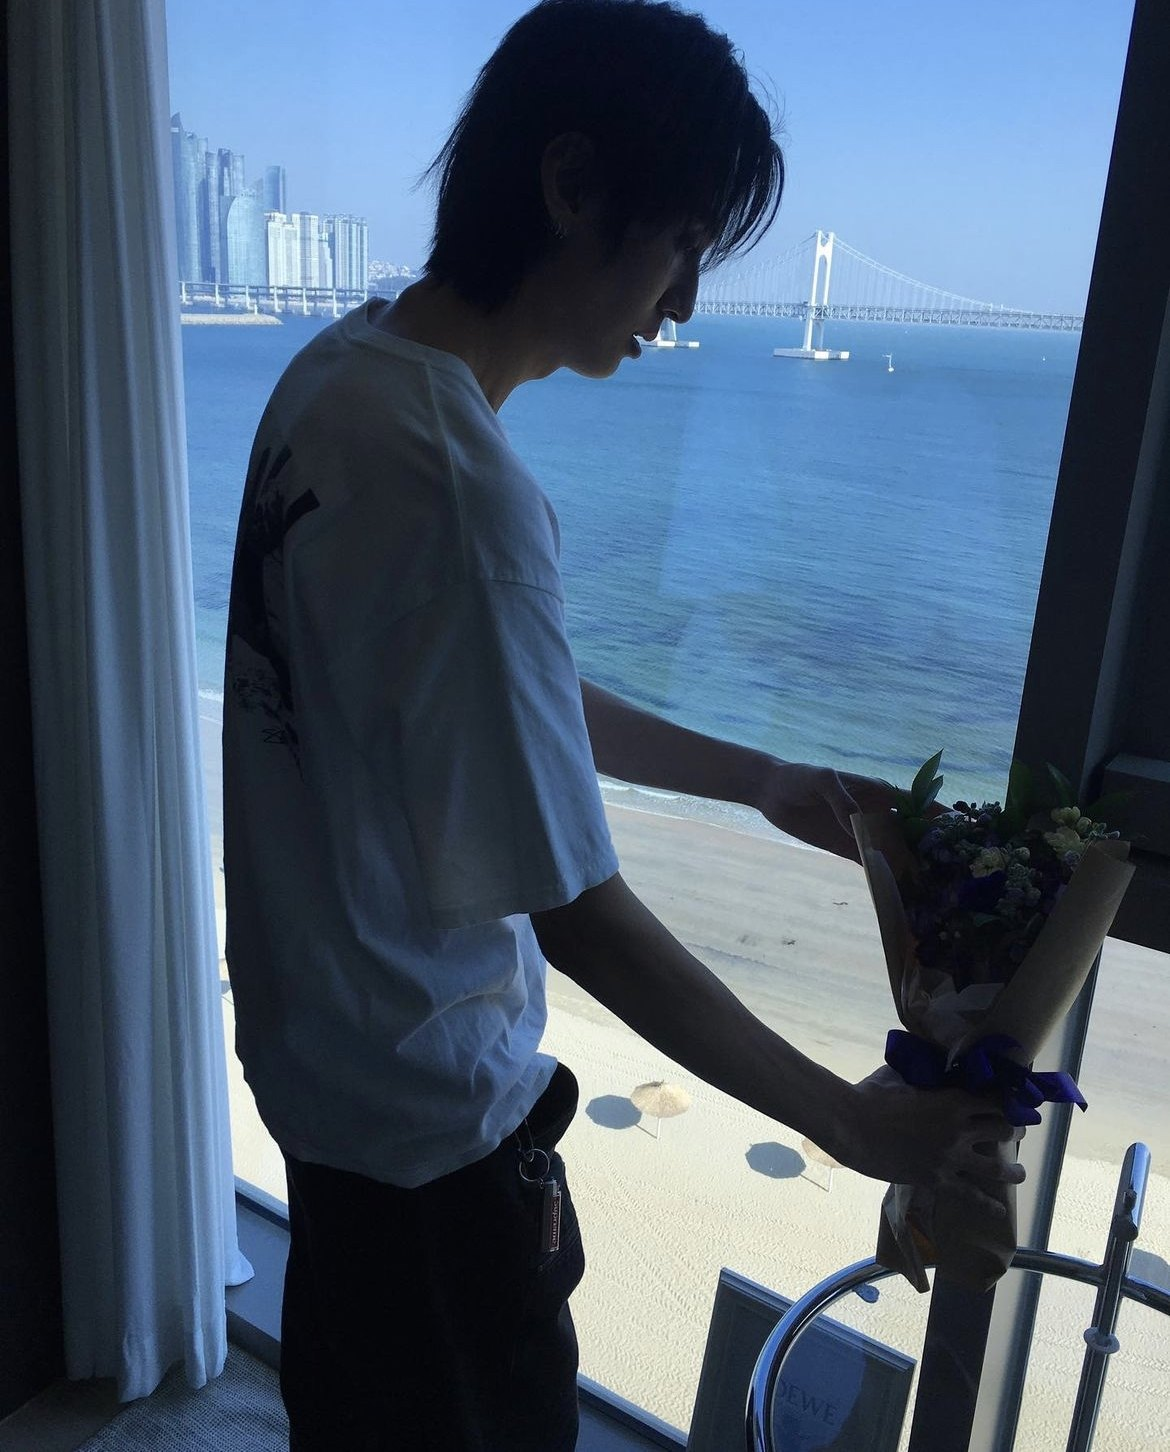
\includegraphics[width=\textwidth]{styled_pics/01.jpg}
        \caption*{Stussy, Y/Project, Supreme}
    \end{figure}
\end{minipage}
\begin{minipage}[h!]{0.5\textwidth}
    \begin{figure}[H]
        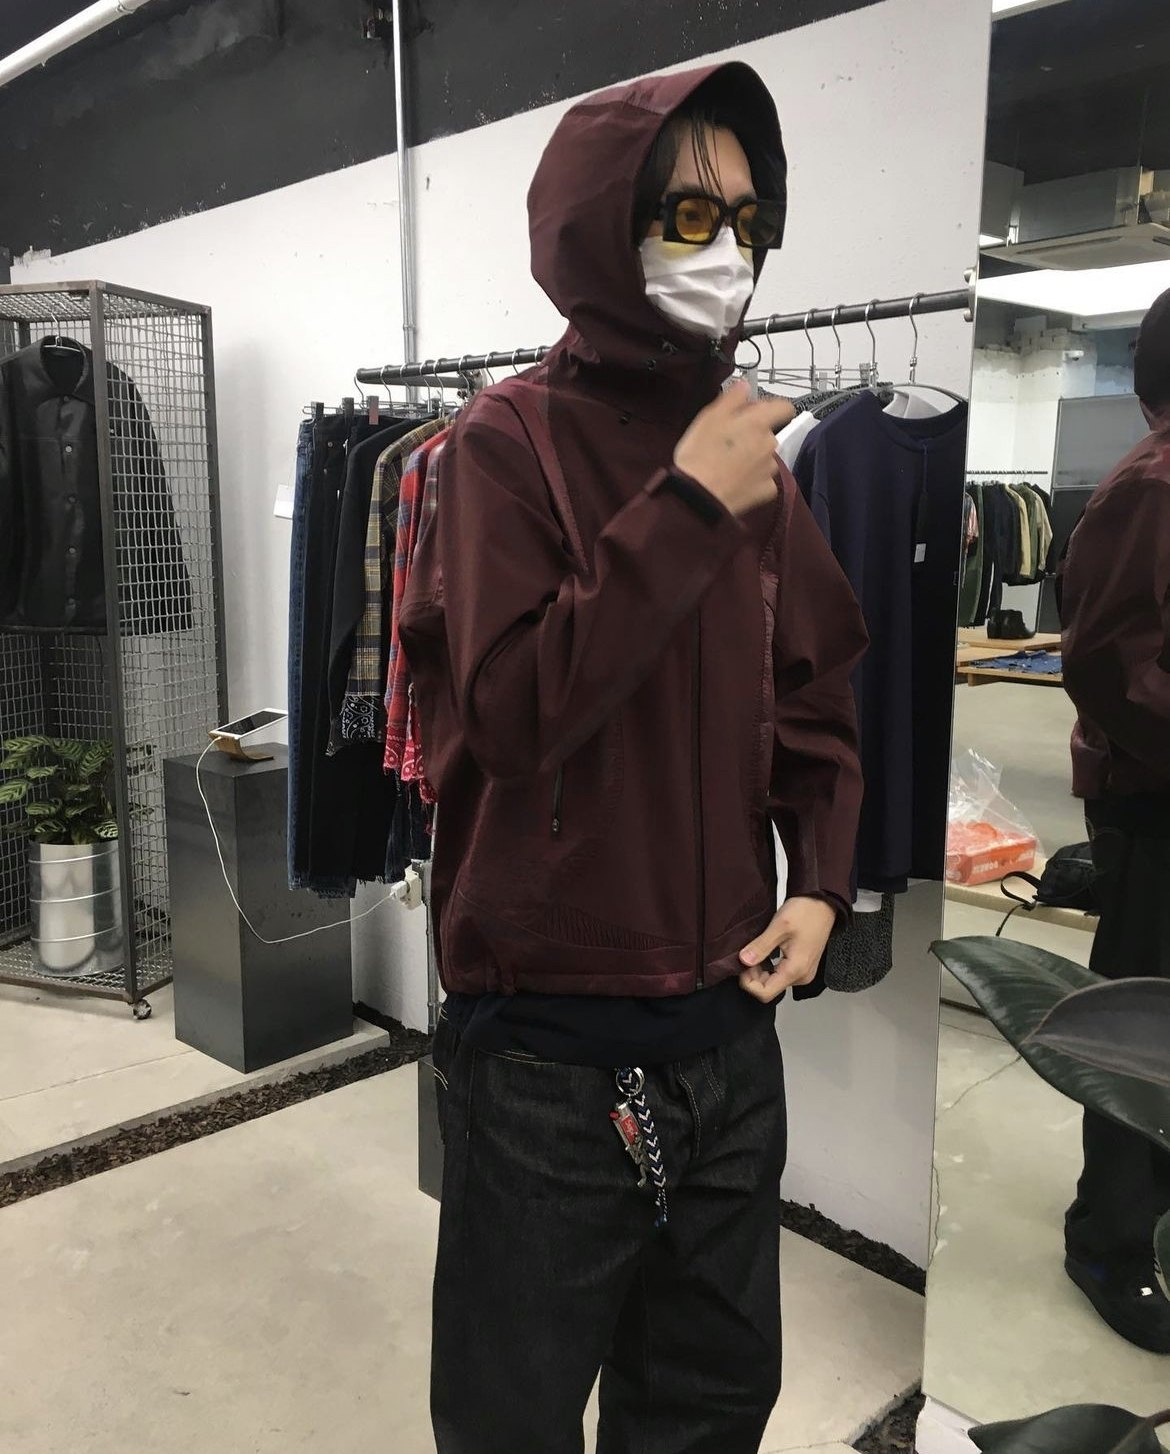
\includegraphics[width=\textwidth]{styled_pics/02.jpg}
        \caption*{XLIM, Levis}
    \end{figure}
\end{minipage}
\begin{minipage}[h!]{0.5\textwidth}
    \begin{figure}[H]
        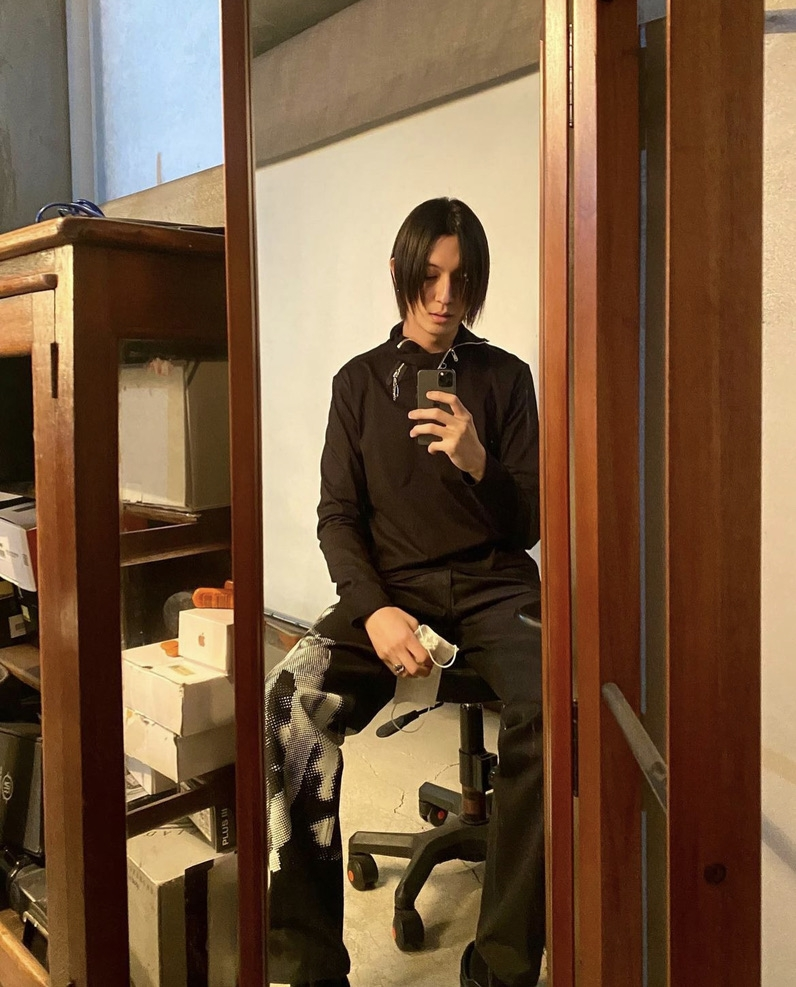
\includegraphics[width=\textwidth]{styled_pics/03.jpg}
        \caption*{TheSoloist., 032c}
    \end{figure}
\end{minipage}
\begin{minipage}[h!]{0.5\textwidth}
    \begin{figure}[H]
        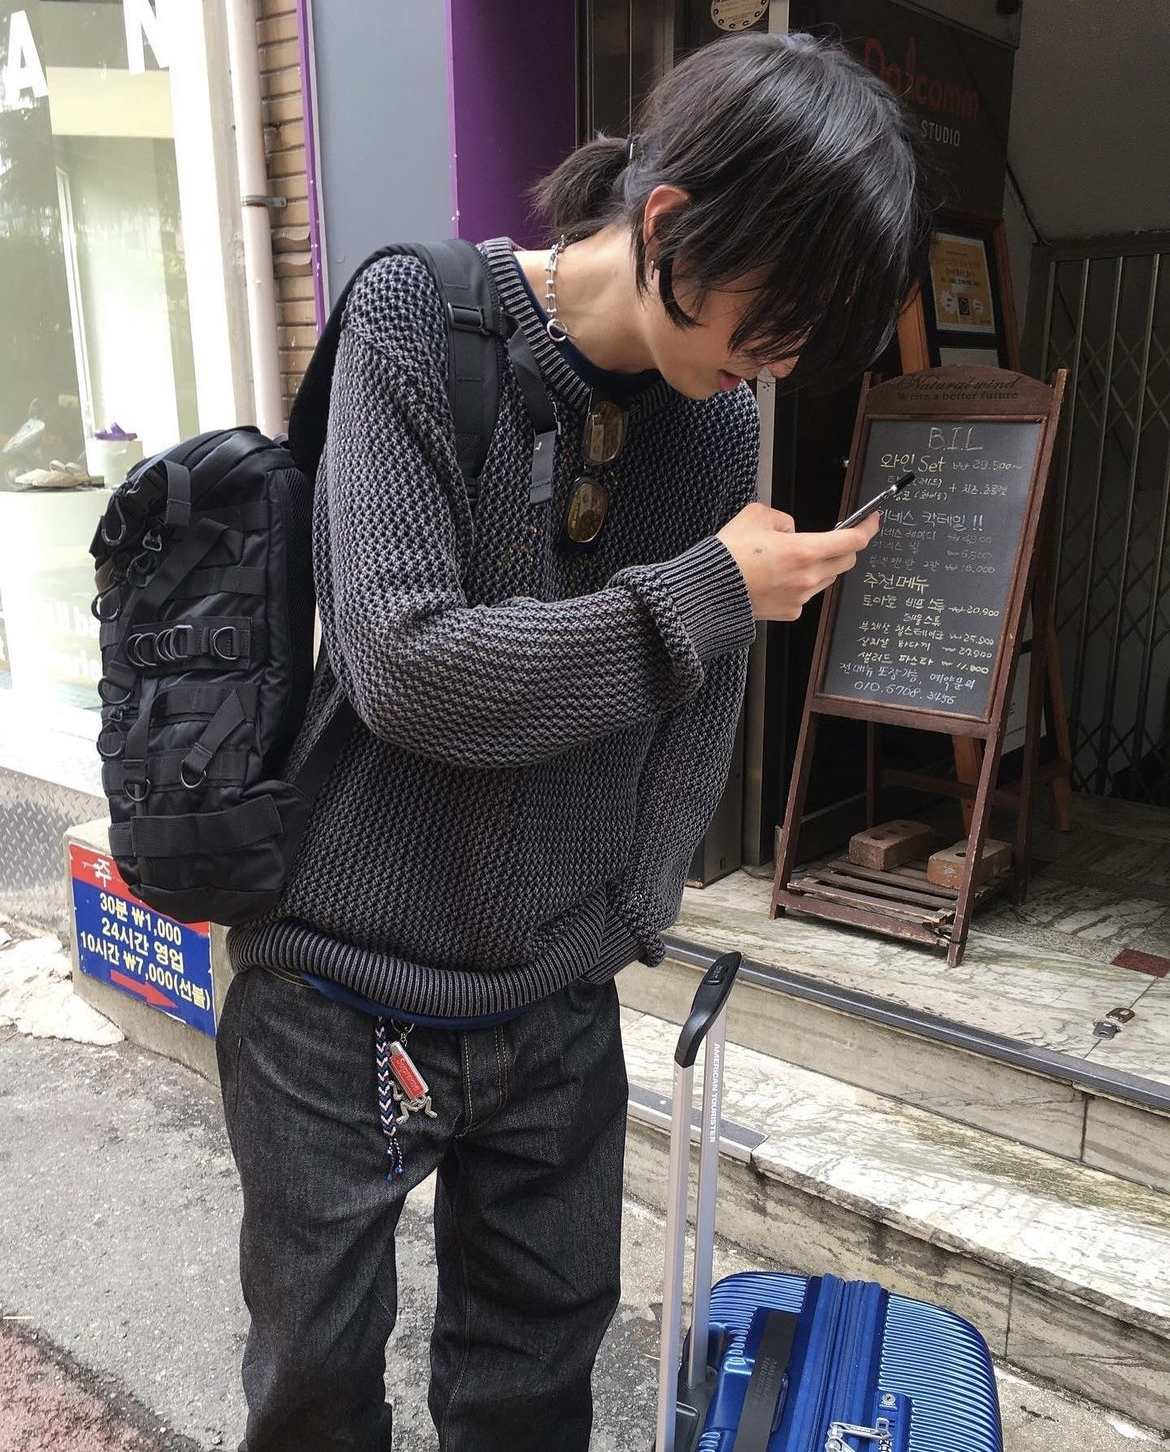
\includegraphics[width=\textwidth]{styled_pics/04.jpg}
        \caption*{032c, Stussy, Levis}
    \end{figure}
\end{minipage}
\begin{minipage}[h!]{0.5\textwidth}
    \begin{figure}[H]
        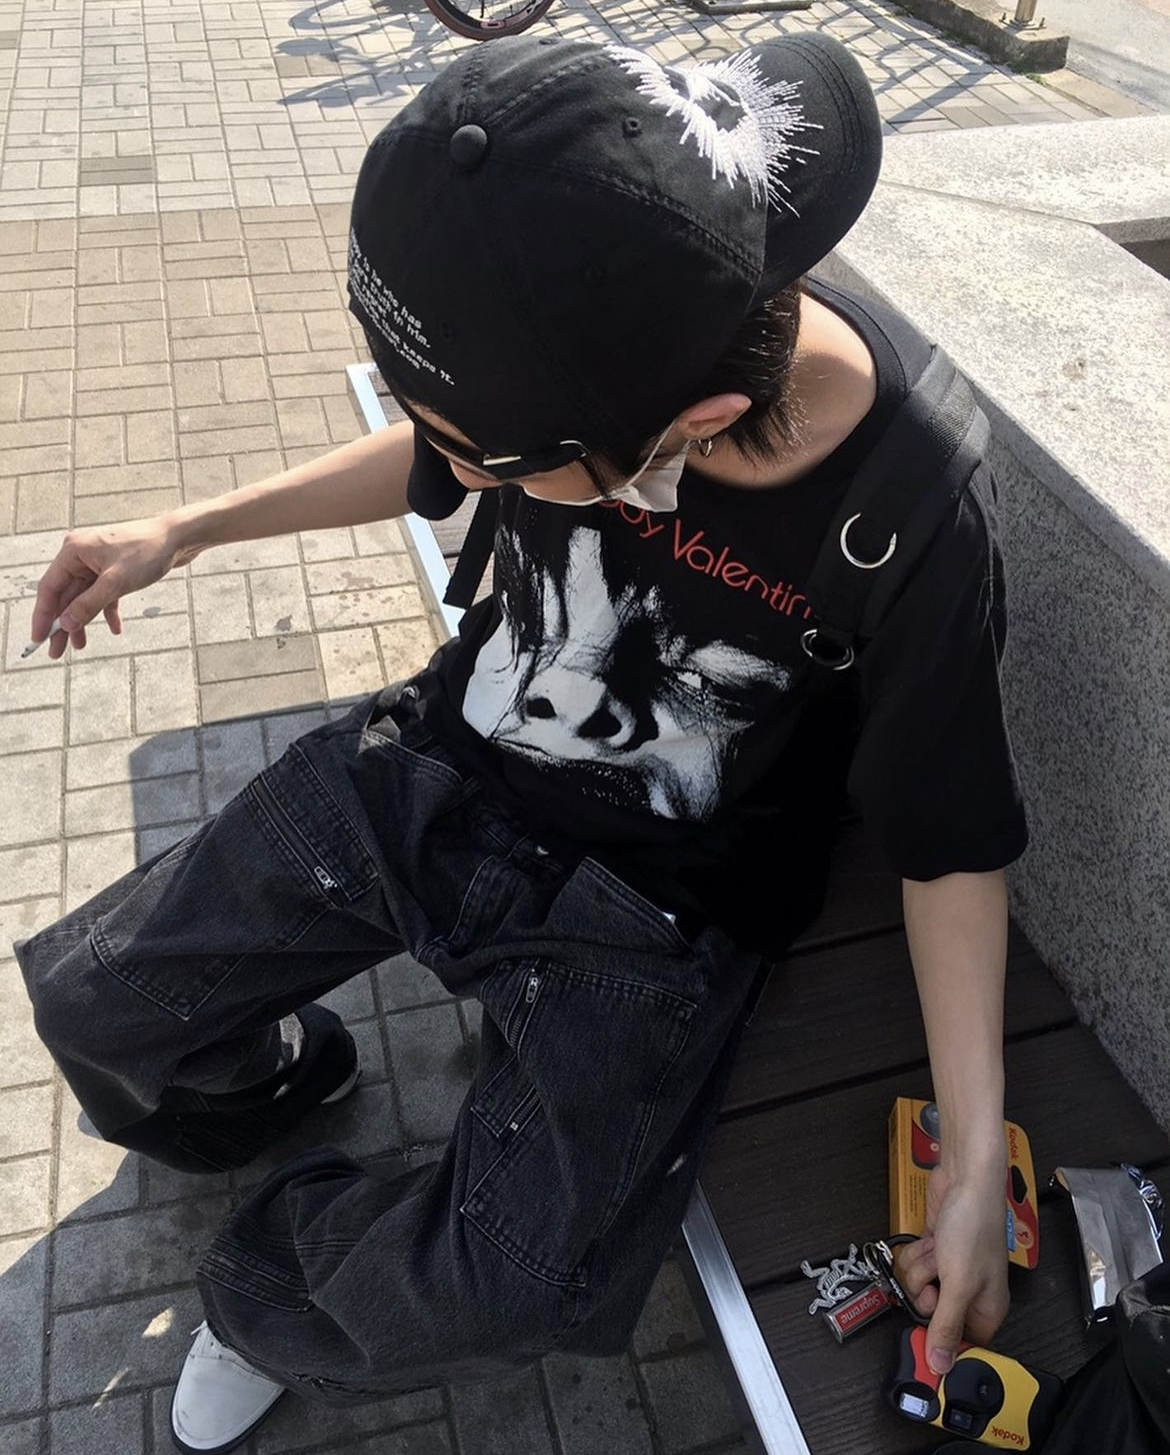
\includegraphics[width=\textwidth]{styled_pics/05.jpg}
        \caption*{Raf Simons, Y/Project, WTAPS}
    \end{figure}
\end{minipage}
\begin{minipage}[h!]{0.5\textwidth}
    \begin{figure}[H]
        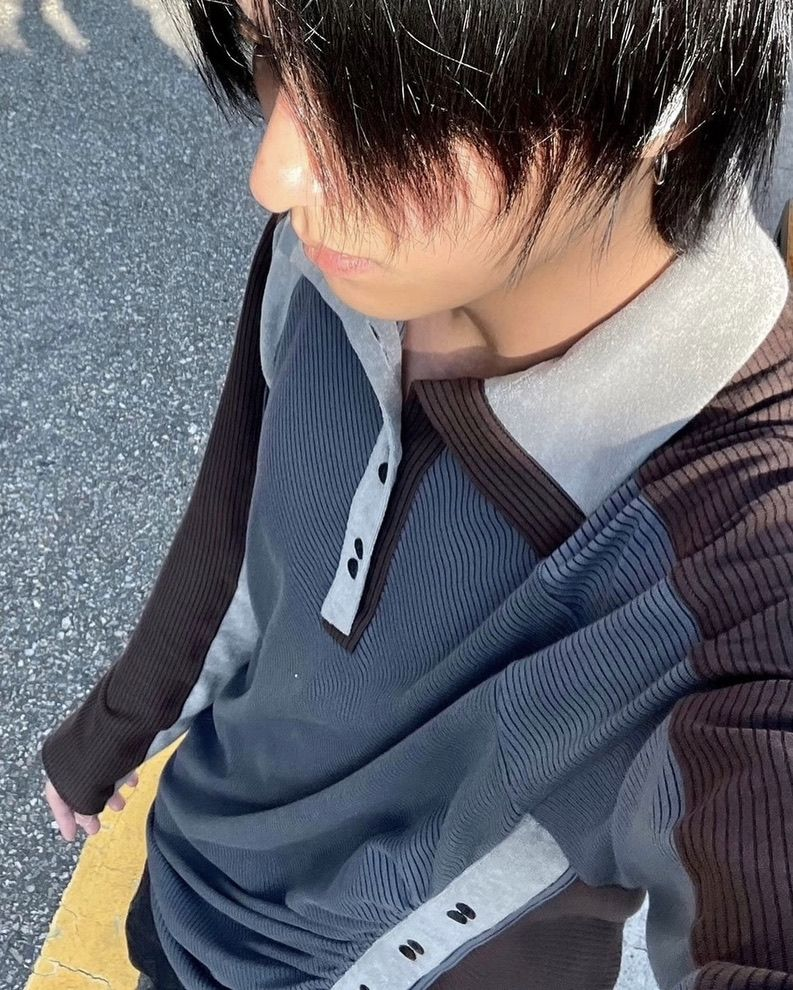
\includegraphics[width=\textwidth]{styled_pics/06.jpg}
        \caption*{Kiko Kostadinov, Namacheko}
    \end{figure}
\end{minipage}
\begin{minipage}[h!]{0.5\textwidth}
    \begin{figure}[H]
        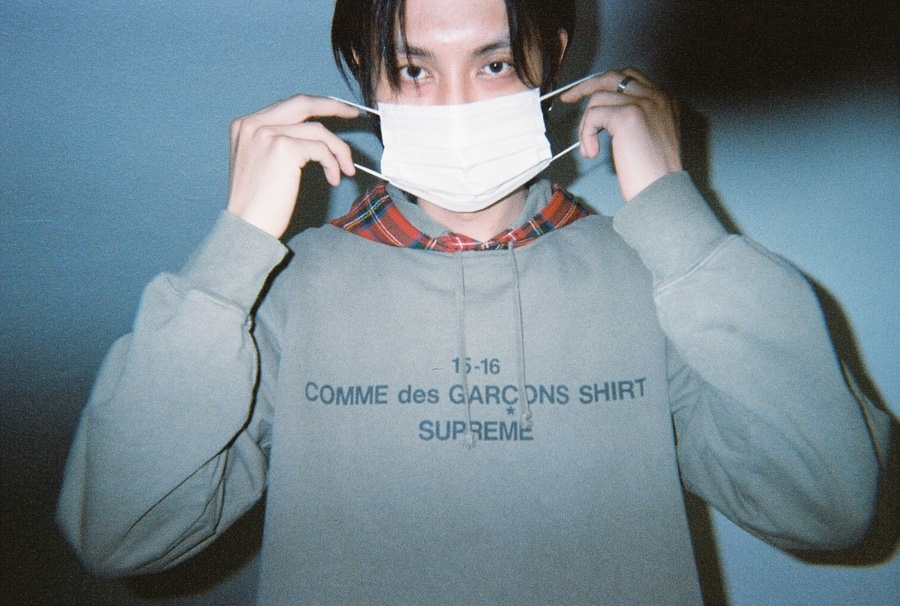
\includegraphics[width=\textwidth]{styled_pics/07.jpg}
        \caption*{Comme des Garcons Shirt, Supreme}
    \end{figure}
\end{minipage}
\begin{minipage}[h!]{0.5\textwidth}
    \begin{figure}[H]
        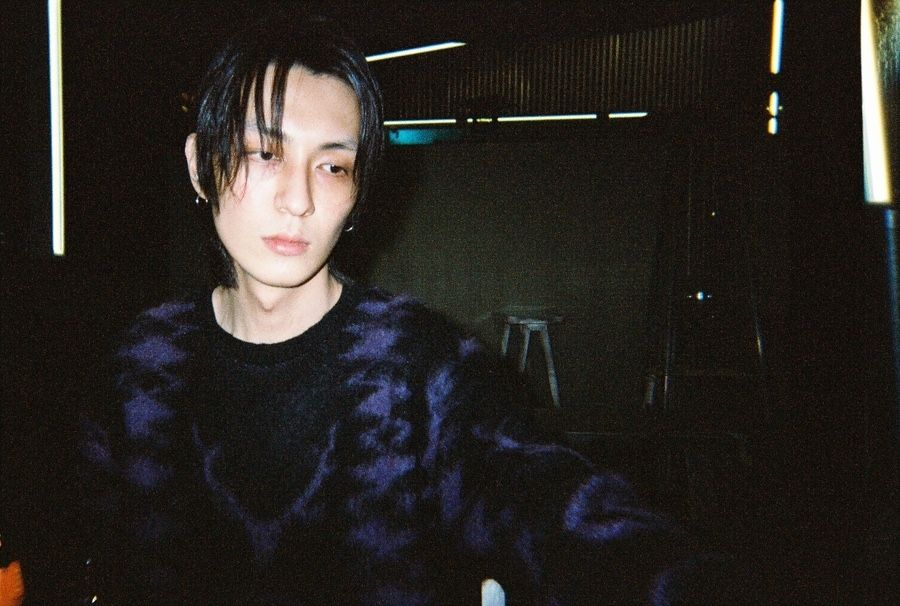
\includegraphics[width=\textwidth]{styled_pics/08.jpg}
        \caption*{South2West8}
    \end{figure}
\end{minipage}
\begin{minipage}[h!]{0.5\textwidth}
    \begin{figure}[H]
        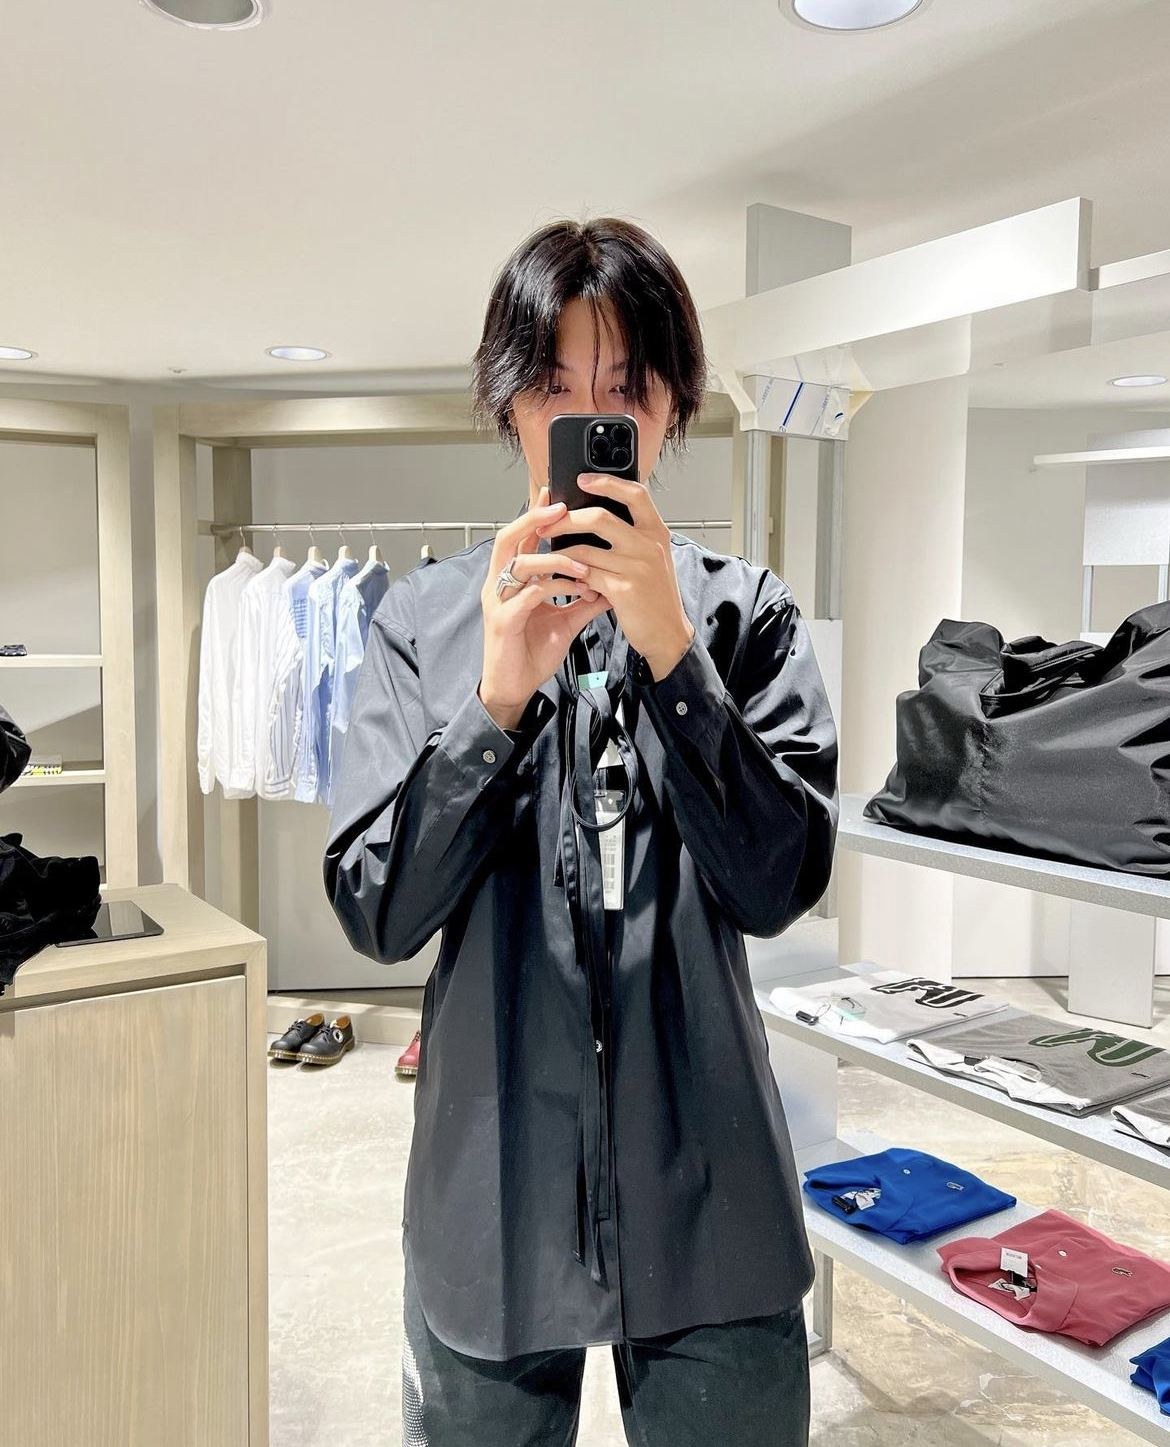
\includegraphics[width=\textwidth]{styled_pics/09.jpg}
        \caption*{Comme des Garcons Shirt, Y/Project}
    \end{figure}
\end{minipage}
\begin{minipage}[h!]{0.5\textwidth}
    \begin{figure}[H]
        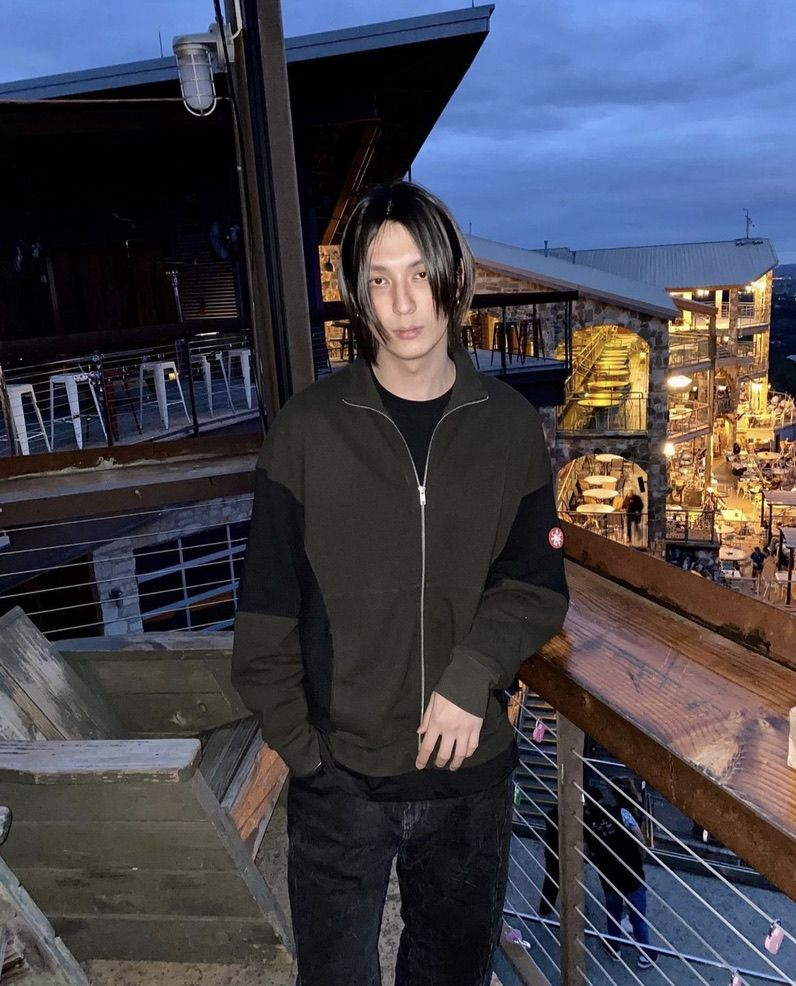
\includegraphics[width=\textwidth]{styled_pics/10.jpg}
        \caption*{Cav Empt, Namacheko}
    \end{figure}
\end{minipage}
\begin{minipage}[h!]{0.5\textwidth}
    \begin{figure}[H]
        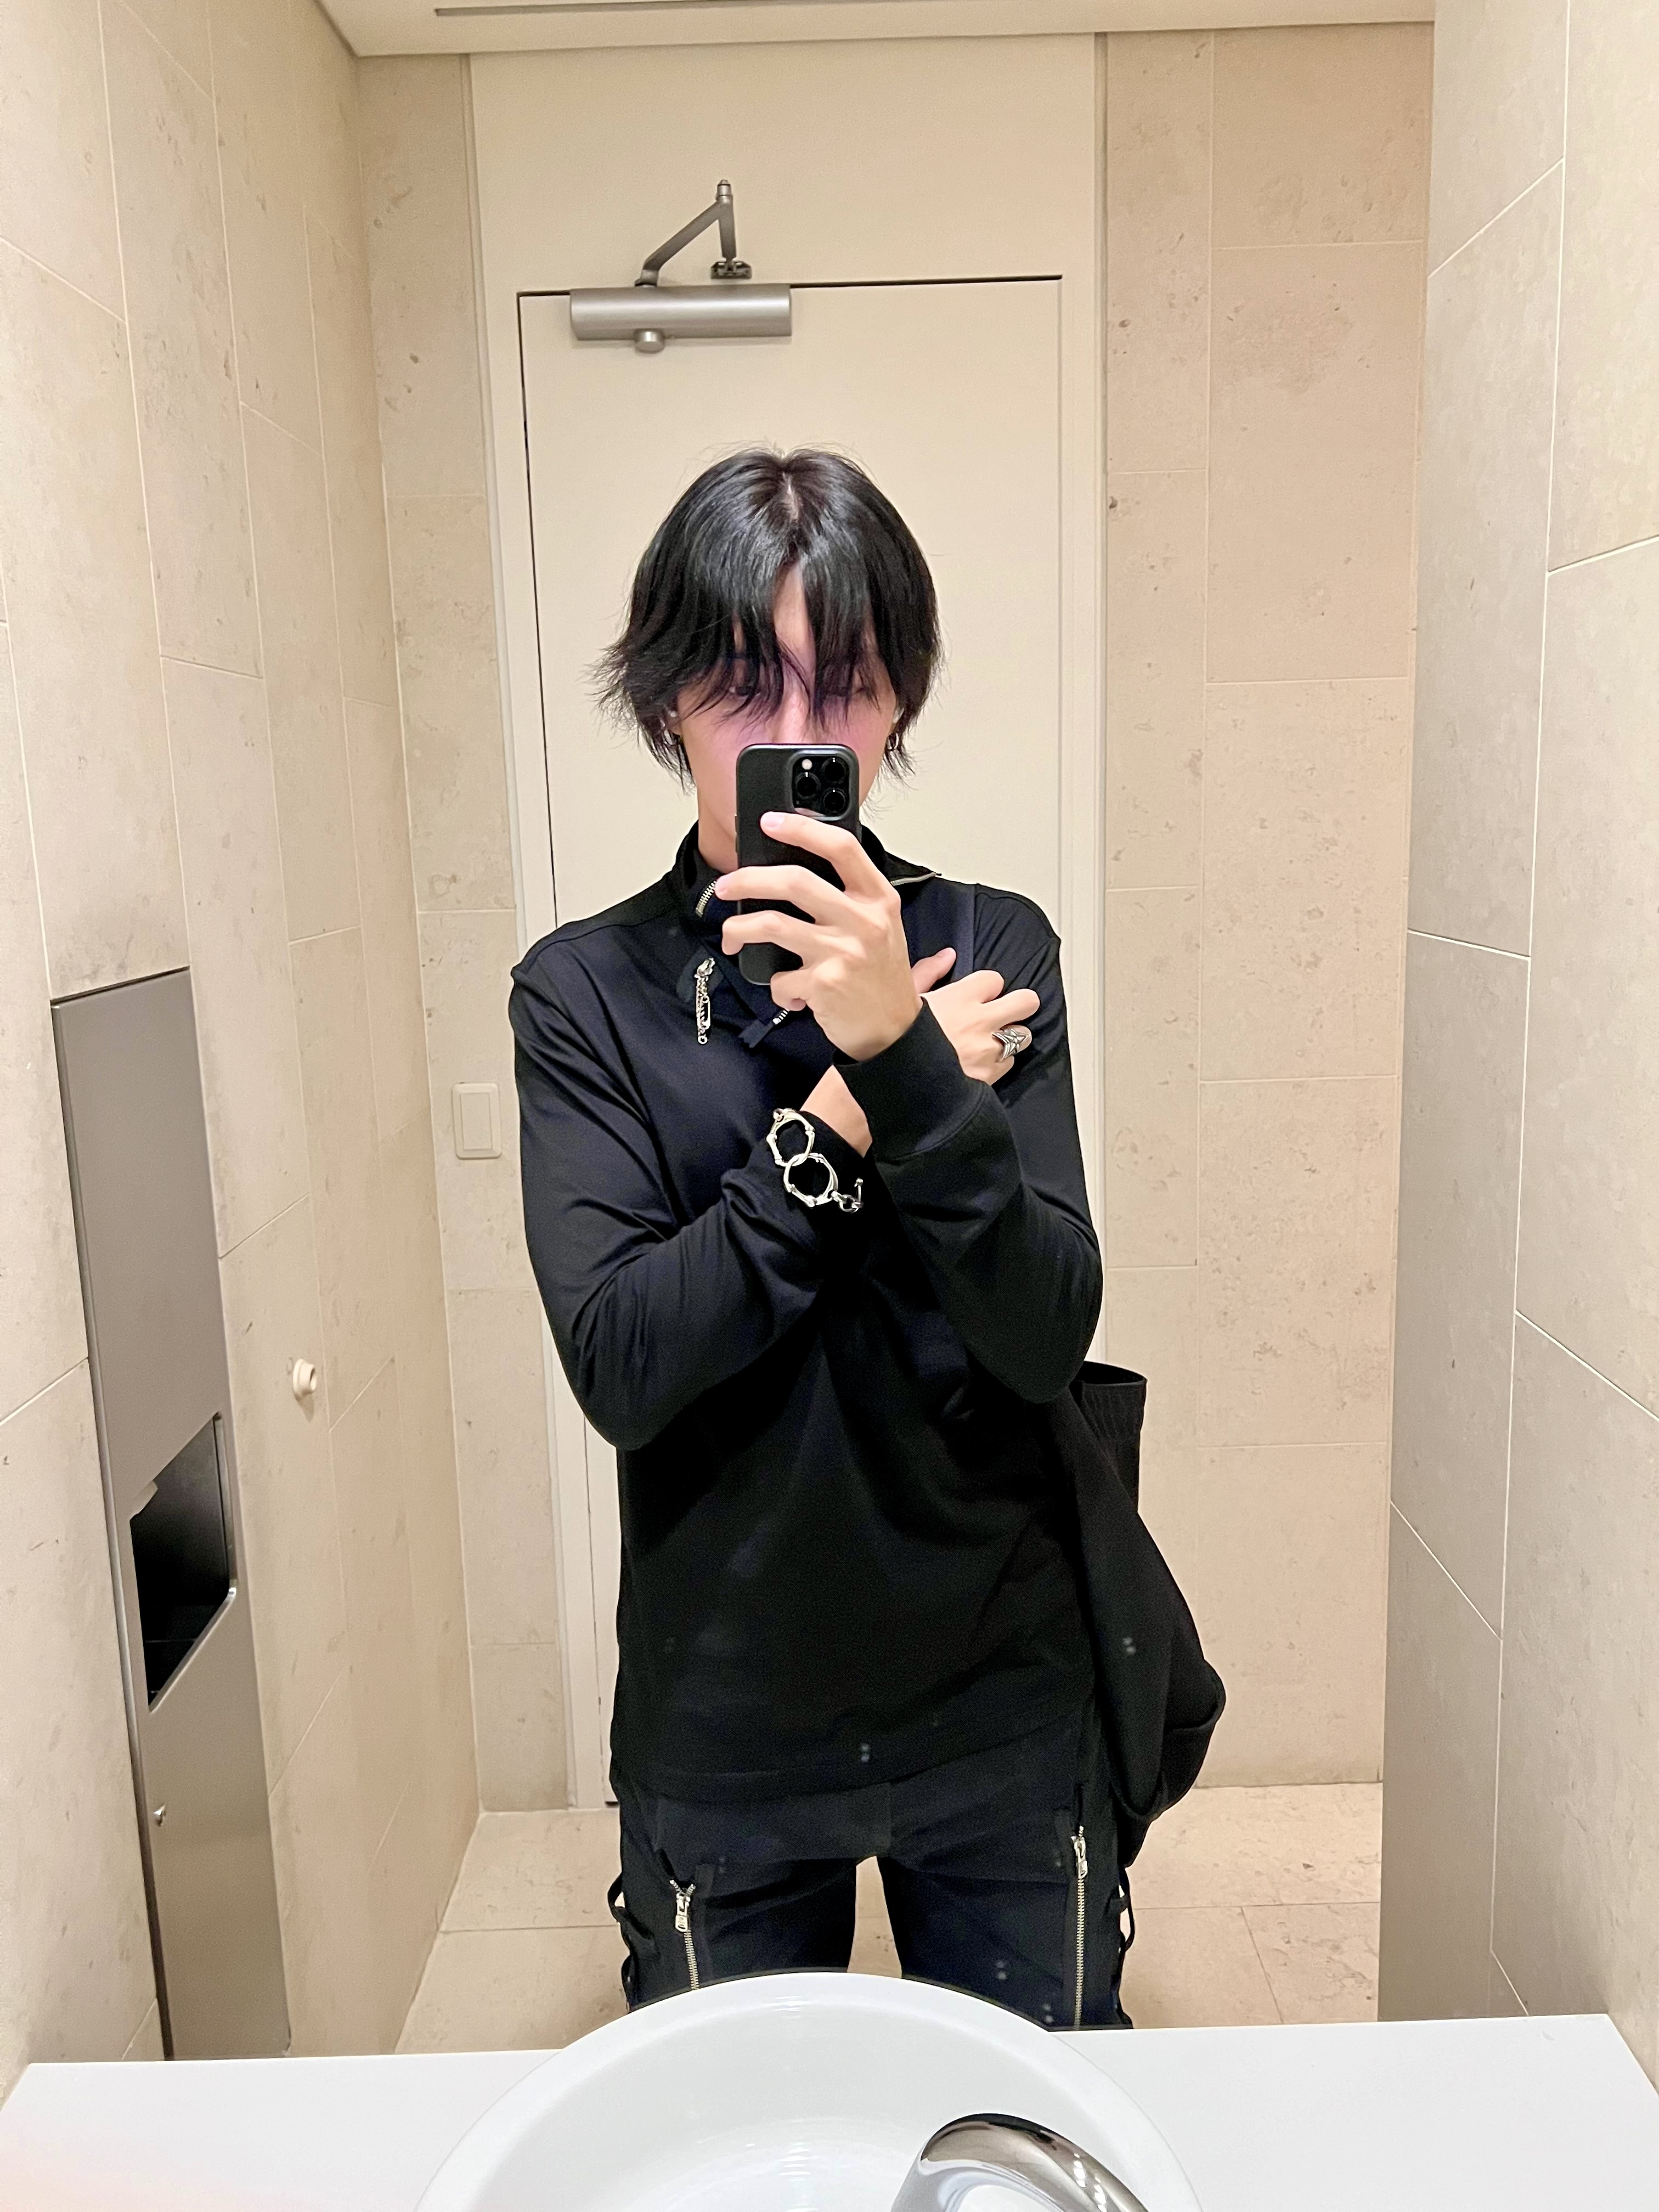
\includegraphics[width=\textwidth]{styled_pics/11.jpg}
        \caption*{Comme des Garcons Homme Plus, TheSoloist.}
    \end{figure}
\end{minipage}
\begin{minipage}[h!]{0.5\textwidth}
    \begin{figure}[H]
        \includegraphics[width=\textwidth]{styled_pics/12.jpg}
        \caption*{Yohji Yamamoto Pour Homme, Y/Project}
    \end{figure}
\end{minipage}
\begin{minipage}[h!]{0.5\textwidth}
    \begin{figure}[H]
        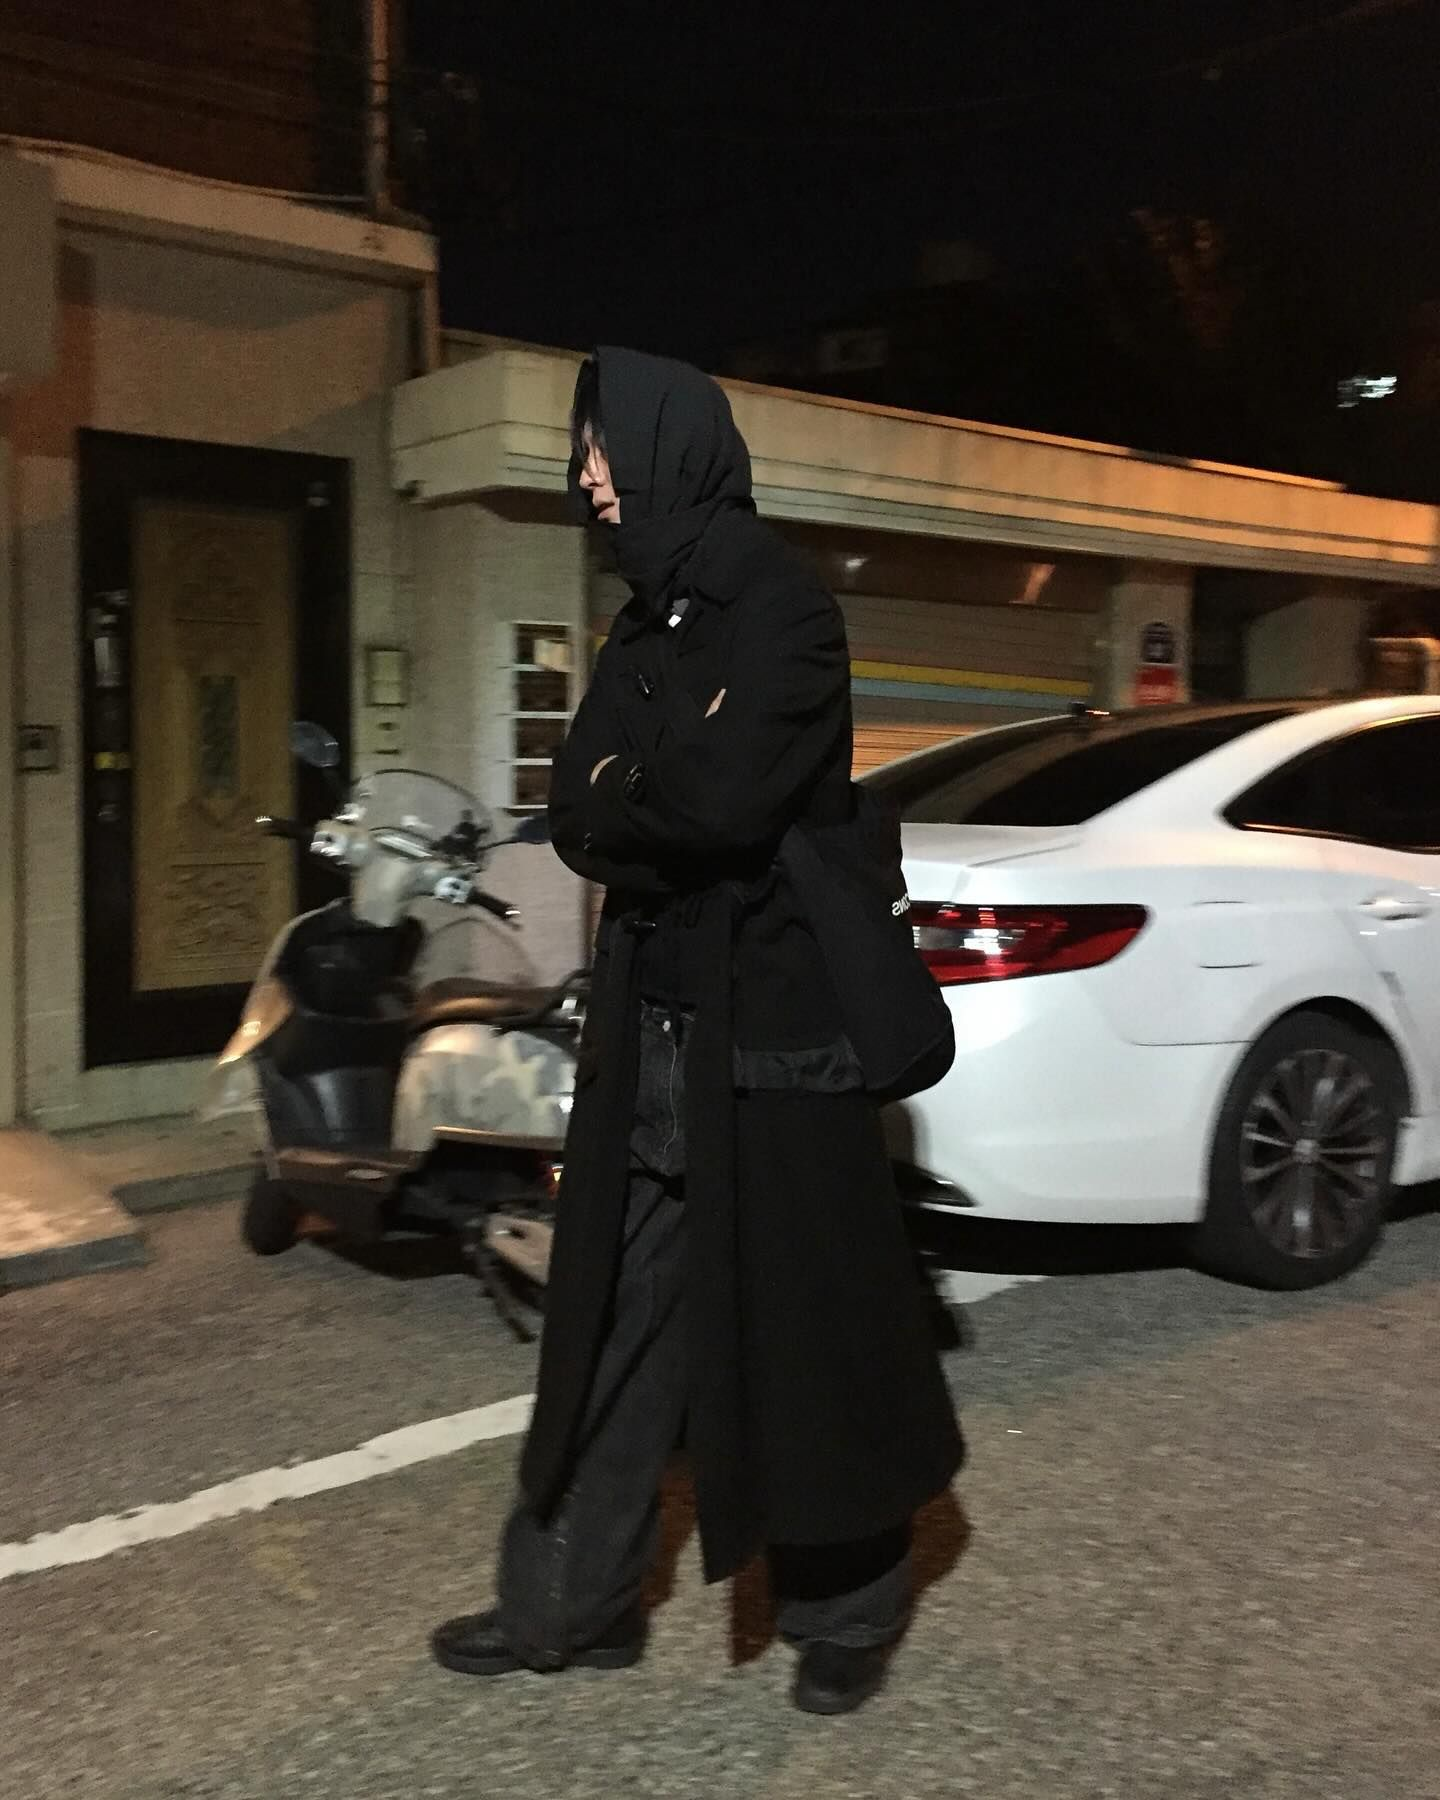
\includegraphics[width=\textwidth]{styled_pics/13.jpg}
        \caption*{Edward Cuming, Craig Green, Comme des Garcons Homme Plus}
    \end{figure}
\end{minipage}
\begin{minipage}[h!]{0.5\textwidth}
    \begin{figure}[H]
        \includegraphics[width=\textwidth]{styled_pics/14.jpg}
        \caption*{GmbH, Comme des Garcons BLACK, 10 Corso Como}
    \end{figure}
\end{minipage}
\begin{minipage}[h!]{0.5\textwidth}
    \begin{figure}[H]
        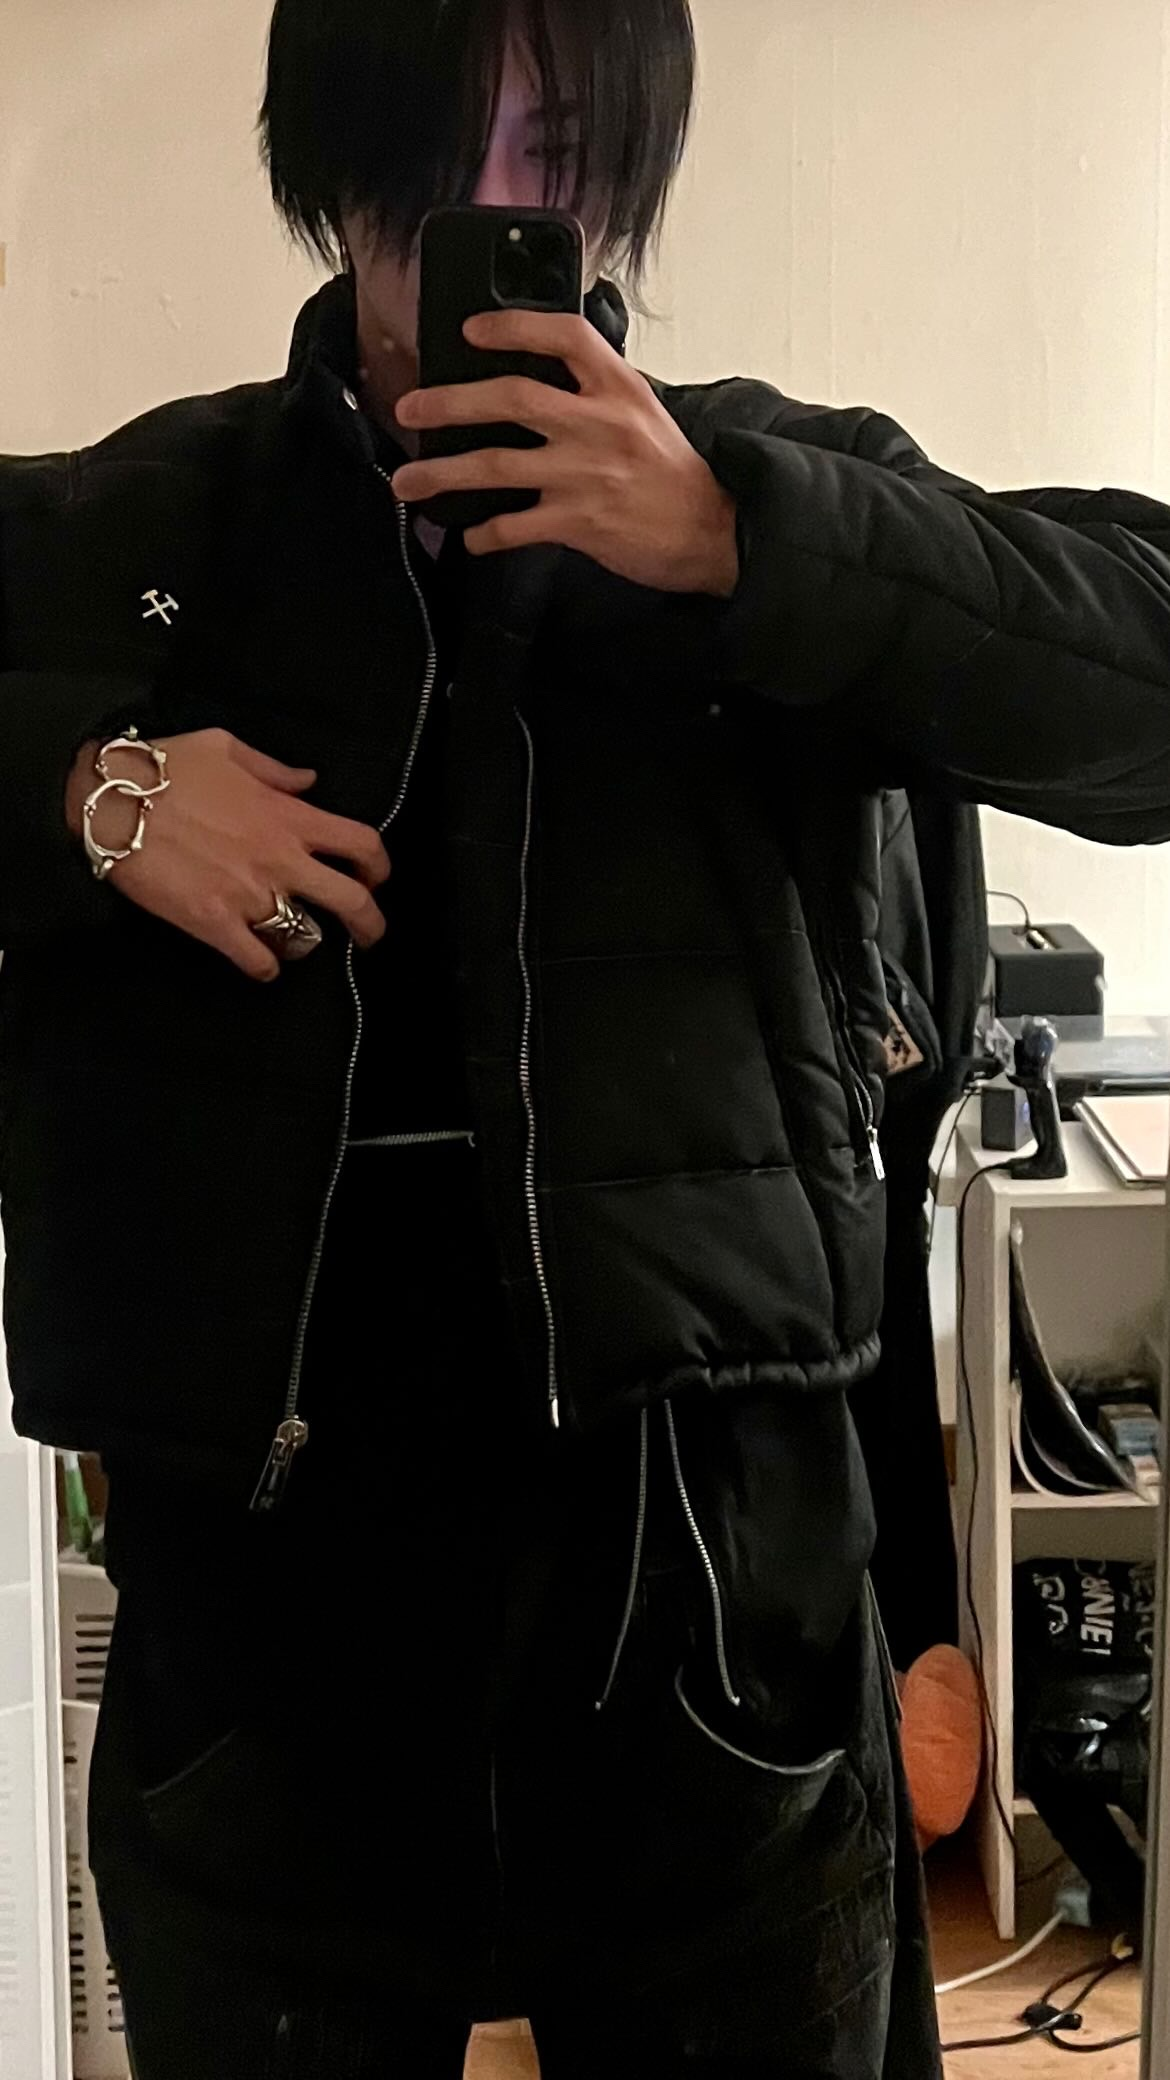
\includegraphics[width=\textwidth]{styled_pics/15.jpg}
        \caption*{Comme des Garcons BLACK, GmbH}
    \end{figure}
\end{minipage}
\begin{minipage}[h!]{0.5\textwidth}
    \begin{figure}[H]
        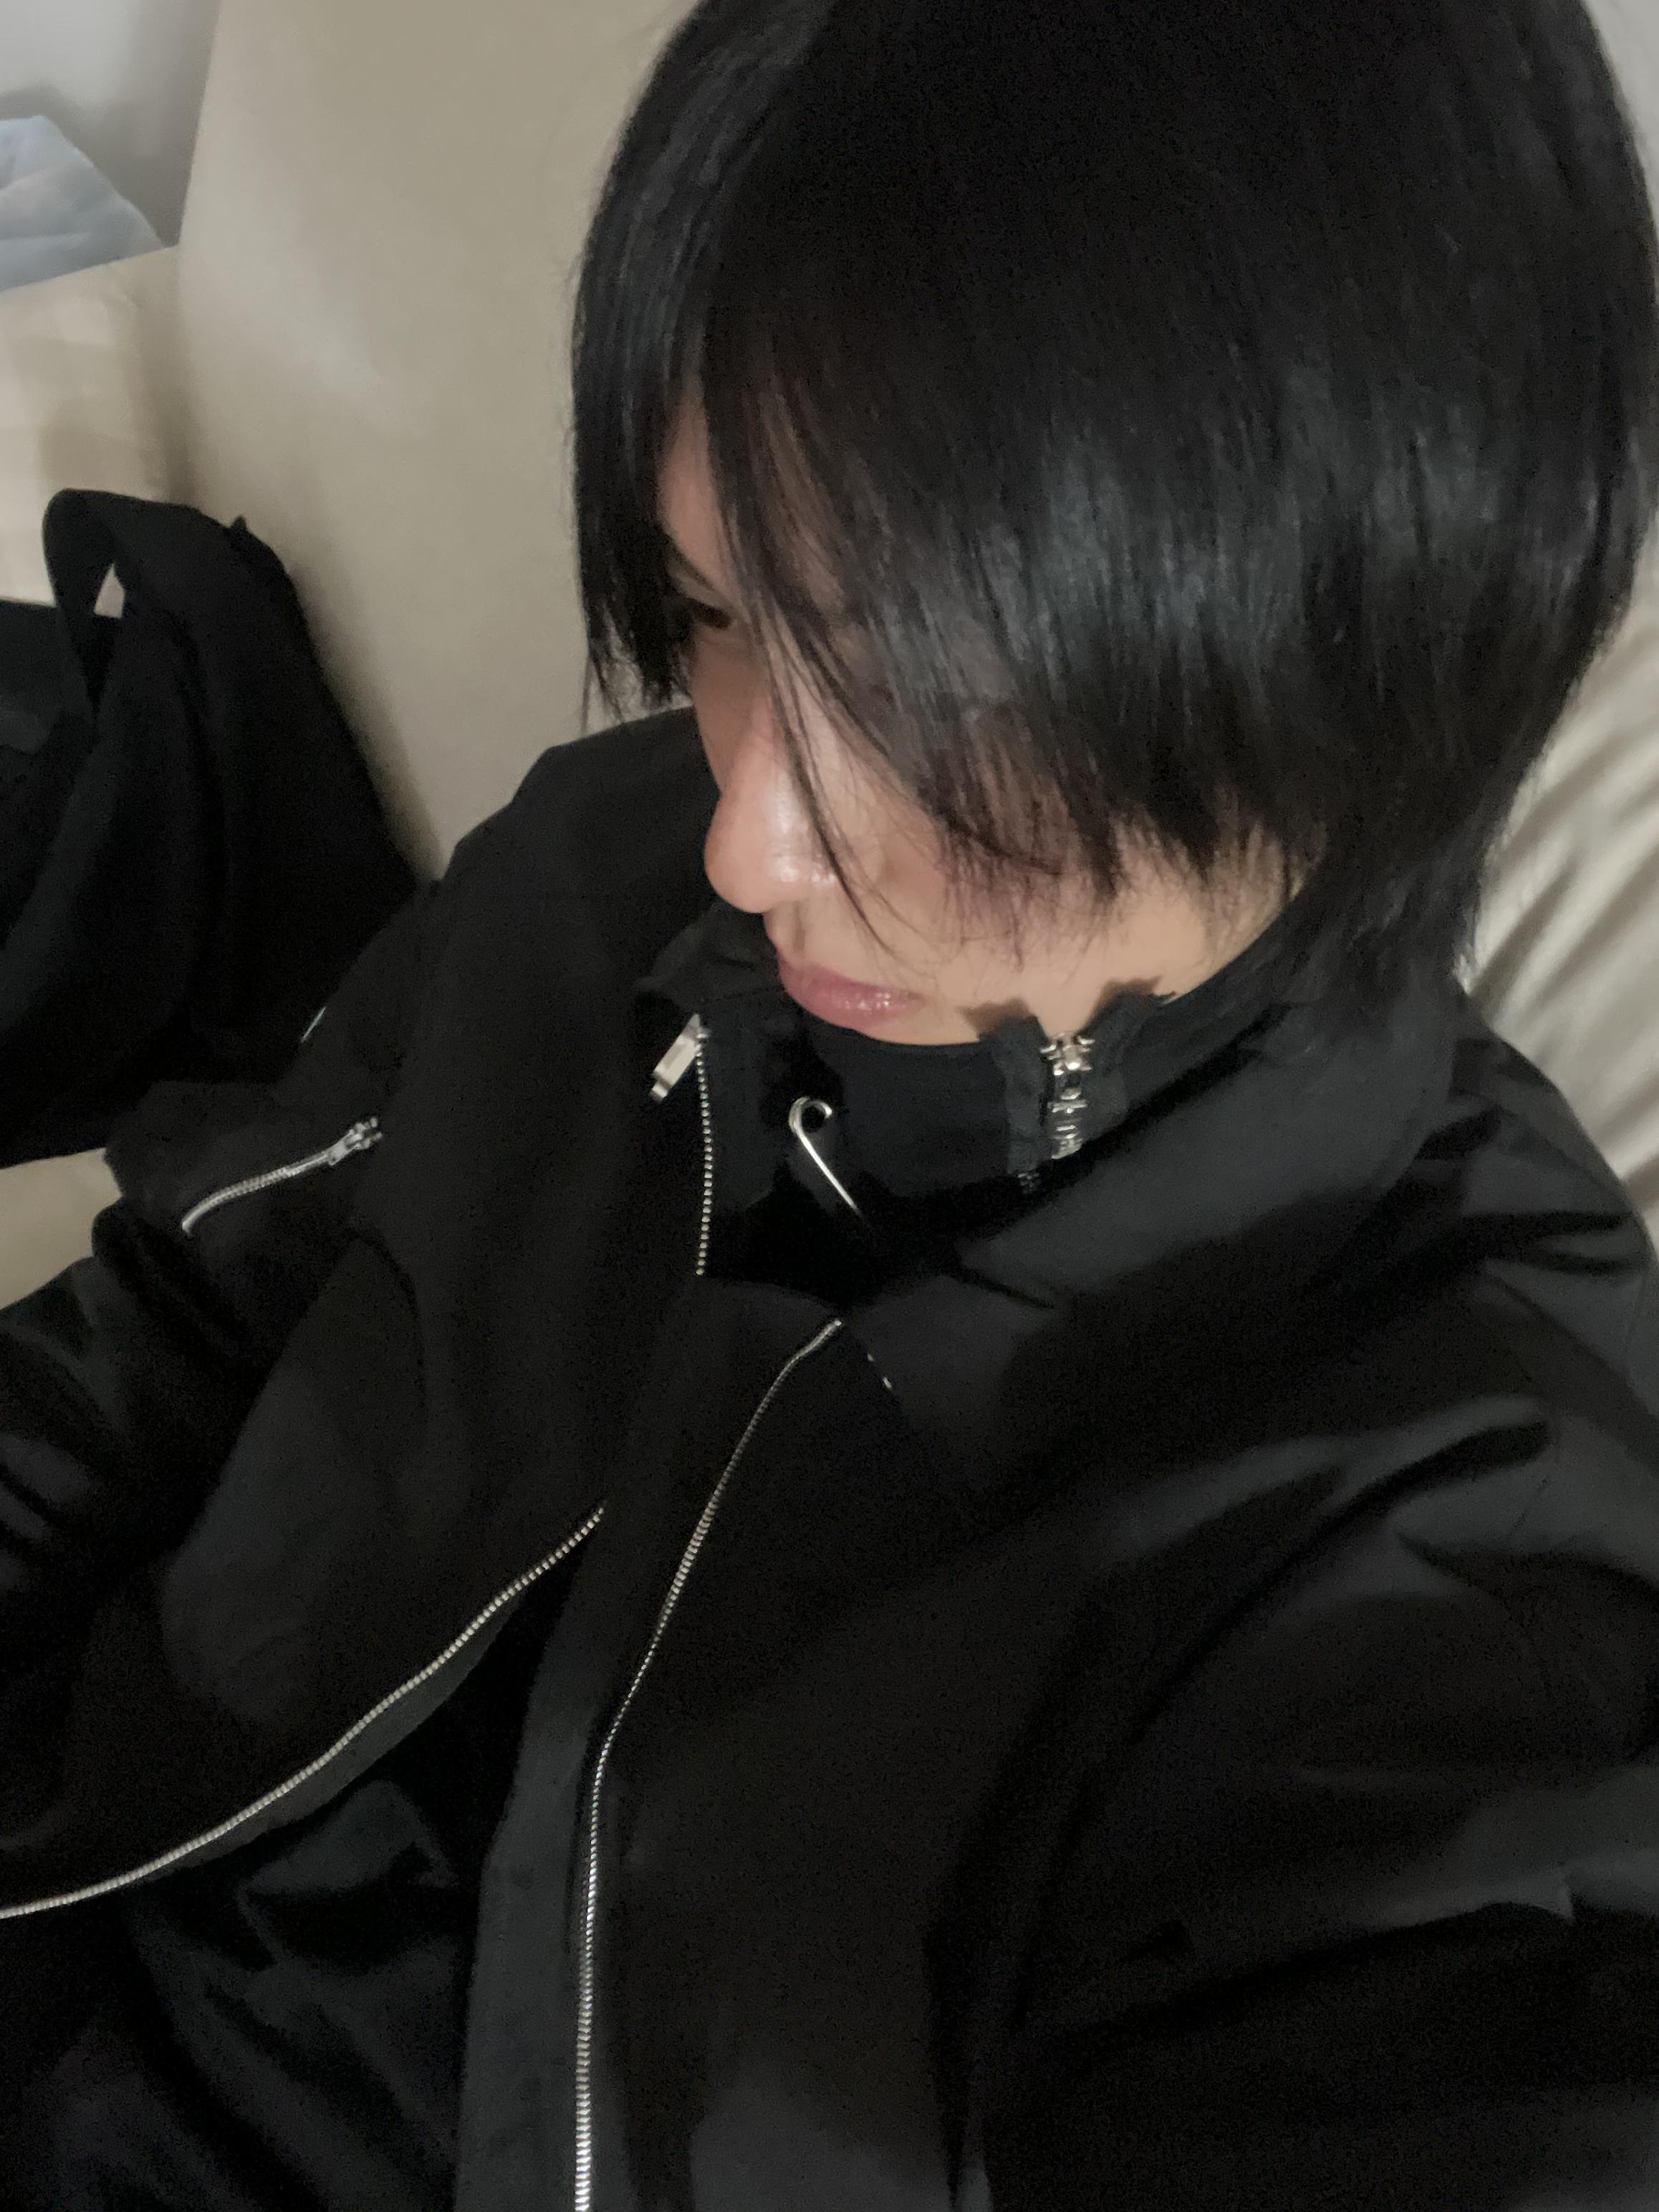
\includegraphics[width=\textwidth]{styled_pics/16.jpg}
        \caption*{1017 ALYX 9SM, TheSoloist.}
    \end{figure}
\end{minipage} 



% End document
\end{document}